\chapter{Algoritmi per SpGEMM esistenti}
\label{Chapter1} % 2 reference \ref{Chapter1} 
%----------------------------------------------------------------------------------------

% Define some commands to keep the formatting separated from the content 
\newcommand{\nnz}{non zero }
\newcommand{\keyword}[1]{\textbf{#1}}
\newcommand{\tabhead}[1]{\textbf{#1}}
\newcommand{\code}[1]{\texttt{#1}}
\newcommand{\file}[1]{\texttt{\bfseries#1}}
\newcommand{\option}[1]{\texttt{\itshape#1}}


\section{Notazione}
Si indica con $C \in \mathbb{R}^{m x n}$ il risultato del prodotto di 
$A \in \mathbb{R}^{m x k},B \in \mathbb{R}^{k x n}$. \\ 
$a_{ij} \in A$ è l'elemento della riga i e colonna j della matrice A.\\
$a_{i*}~,~a_{*j}$ indicano rispettivamente la riga i-esima e la colonna j-esima della matrice A\\
$I_i(A)$ indica il set di indici di colonna relativi agl'elementi non zero della riga i-esima di A\\
$I_j(B)$ indica il set di indici di riga relativi agl'elementi non zero della colonna j-esima di B\\
$I(i,j)$ indica il set di indici $k$ di righe di A e di colonne di B tali che
$a_{ik}*b_{kj} \neq 0$\\
$nnz(A)$ indica il numero di non zeri della matrice A. \\ 
$nzc(A)~,~nzr(A)$ indicano rispettivamente il numero di colonne e di righe di A 
con almeno un elemento \nnz.\\

\section{Formulazioni SpGEMM}
Gli algoritmi per la risoluzione del prodotto tra due matrici sparse possono
essere classificati in base alle formulazioni e partizionamento dei dati del problema SpGEMM 
\parencite{sysReviewChi}.\\ Le principali formulazioni del problema sono sono:
\begin{itemize}
  \item Inner-product \qquad $c_{ij} = \sum\limits_{k \in I(i,j)}  a_{ik} \ast  b_{kj}$
  \item Outer-product \qquad $C = \sum\limits_{i=1}^k  a_{*i} \otimes  b_{i*}$		
  \item row-by-row	  \qquad $c_{i*} = \sum\limits_{k \in I_i(A)}  a_{ik} \ast  b_{k*}$
  \item col-by-col    \qquad $c_{*j} = \sum\limits_{k \in I_j(B)}  a_{*k} \ast  b_{kj}$
\end{itemize}

\subsection{Rappresenzione mediante grafi}
Le formulazioni per GEMM possono essere rappresentate graficamente mediante
grafi a 3 strati U, W, V \parencite{2dNewIdeas,cohen3LayeredGraphs} dove:
\begin{itemize}
  \item i nodi in $U \ni u_i$:   rappresentano le righe di A
  \item i nodi in $V \ni v_j$:   rappresentano le colonne di B
  \item i nodi in $W \ni w_k$:   rappresentano la dimensione in comune tra A e B
\end{itemize}
esiste un arco $(u_i,w_l) ~ \forall ~ a_{i,l} \neq 0$\\
esiste un arco $(w_l,v_j) ~ \forall ~ b_{l,j} \neq 0$\\
%%TARGET GRAPH RAPPR
Per ogni formulazione di SpGEMM, l'obbiettivo è quello di trovare coppie di
vertici $(u_i,v_j)$ connessi da un nodo comune $w_k$ e unire i
contributi di coppie di vertici che condividono nodi adiacenti\\ %TODO

%%INNER PRODUCT
\begin{figure}[h]
  \centering \includegraphics{layeredGraphInnerProduct.svg.png} 
  \caption[Rappresentazione grafica del calcolo di $c_{i,j}$ mediante Inner-product]
  \decoRule \label{fig:layeredGraphInnerProduct}
\end{figure}
Per la formulazione Inner-product \ref{fig:layeredGraphInnerProduct} 
è necessario esaminare ogni coppia di vertici  in U e V per trovare 
il sottoinsieme di $\tilde{W_{ij}} \subseteq W$ che connette coppie di nodi. \\
Vengono accumulati i prodotti $a_{il} \cdot b_{lj}$ relativi a $\tilde{W_{ij}}$ in $c_{ij}$.\\
È possibile osservare come la sparsità delle matrici non è sfruttata dato
che è necessario analizzare tutte le coppie di nodi $(u_i,v_j)$\\
%%OUTER PRODUCT
\begin{figure}[h]
  \centering 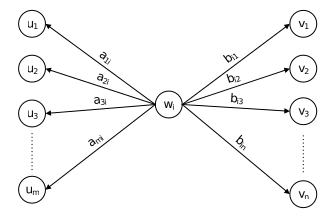
\includegraphics{layeredGraphOuterProduct.svg.png} 
  \caption[Rappresentazione grafica della componente $a_{*i} \cdot b_{i*}$ del calcolo di C mediante Outer-product]
  \decoRule \label{fig:layeredGraphOuterProduct}
\end{figure}
Per la formulazione Outer-product \ref{fig:layeredGraphOuterProduct}
è possibile identificare le coppie di vertici connesse a
partire dai nodi di W che, per matrici sufficientemente sparse,
può essere un operazione più veloce rispetto all'Inner-product.\\
%TODO si complica l'accumulazione dei risultati intermedi
%%row-by-row
\begin{figure}[h]
  \centering 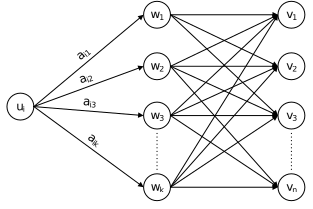
\includegraphics{layeredGraphRowByRow.svg.png} 
  \caption[Rappresentazione grafica della componente $a_{i*} \cdot B$ del 
     calcolo di C mediante formulazione row-by-row]
  \decoRule \label{fig:layeredGraphRowByRow}
  
\end{figure}
Per la formulazione Row-by-row \ref{fig:layeredGraphRowByRow}
le coppie di vertici d'interesse per il risultato di C sono identificabili 
a partire da attraversamenti del grafo indipendenti a partire dai vertici di U verso V.\\
%%col-by-col
Nel caso col-by-col vi è un attraversamento del grafo dai nodi di V a U, 
isomorfico rispetto al caso Row-by-row\\



\section{Algoritmi}
%%SRC STUDIES = Gustavson
Molte delle ricerche riguardo SpGEMM sono basate sull'algoritmo di Gustavson \parencite{gustavson},
un algoritmo sequenziale basato sulla formulazione Row-by-row, riportate in forma di pseudo-codice 
in \ref{figCode:gustavsonRigheSysSurvey} e graficamente in \ref{fig:gustavsonRigheGraphicalIntel}.\\

\begin{figure}[h]
  \caption[pseudo-codice dell'algoritmo di Gustavson]
  \centering 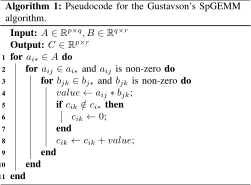
\includegraphics{gustavsonRigheSysSurvey.svg.png} \decoRule
  \label{figCode:gustavsonRigheSysSurvey}
\end{figure}
\begin{figure}[h]
  \caption[rappresentazione grafica di una iterazione dell'algoritmo di Gustavson]
  \centering 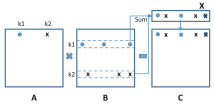
\includegraphics{gustavsonRigheGraphicalIntel.svg.png} \decoRule
  \label{fig:gustavsonRigheGraphicalIntel}
\end{figure}
È possibile notare come nell'algoritmo vi sia l'esigenza di accumulare le righe
risultanti della matrice C. Meccanismi efficienti per realizzare questa
funzionalità sono analizzati successivamente in \ref{ssec:gustavsonDerivate} %TODO FIX REF
\\


\section{Algoritmi paralleli multi-dimensionali}
Gli algoritmi paralleli risolutivi del prodotto tra matrici possono essere
classificati in base al partizionamento del carico di lavoro sui processi.\\
\begin{figure}[h]
  \centering \includegraphics{pGEMM_cube.svg.png} 
  \caption[Rappresentazione grafica dell'assegnamento dei task per la risoluzione
      di SpGEMM in 1,2 e 3 dimensioni]\decoRule \label{fig:pGEMM_cube}
\end{figure}
%%WORKCUBE INTRO
L'assegnamento dei sotto problemi può essere visualizzato in un cubo di lavoro W \ref{fig:pGEMM_cube}
in cui ogni moltiplicazione di elementi \nnz $a_{i,k}*b_{k,j}$ è rappresentabile
con voxel $W(i,j,k)$ \parencite{cartesianPartitioningModels}.
Le proiezioni $W(i,j,k)$  sulle facce del cubo relative alle matrici A e B 
hanno elementi \nnz e determinano il pattern degl'elementi \nnz sulla matrice C.
%WORKCUBE NOTATIONS
I sottoinsiemi dei voxel di W ottenuti fissando uno o due indici sono denominati:
\begin{itemize}
  \item Layers: W(i,:,:),W(:,j,:),W(:,:,k)
  \item Fibers: Intersezioni di Layers relativi a indici diversi, e.g. W(i,j,:)
  \item Cuboid: Sottoinsiemi di W con tutte le dimensioni minori delle 
   dimensioni delle matrici corrispondenti
\end{itemize}

\subsection{Matrici ipersparse e rappresentazione DCSC}
È possibile definire una matrice sparsa A, come {\bf ipersparsa }se $nnz(A)$ è
inferiore alla sua dimensione più grande N\\ %TODO def in newIdeas 14.2.2, matrici quadrate
Le matrici ipersparse sono rare nell'algebra lineare numerica ma occorrono 
frequentemente nel processamento grafi, particolarmente se in parallelo.\\

Inoltre, data una suddivisone bidimensionale di una matrice sparsa, %TODO quadrata
per un processamento parallelo in una griglia di p processi, si ha che ogni processo
verrà assegnato ad una matrice di dimensione $(n/\sqrt{p})~x~(n/\sqrt{p})$.
L'occupazione globale di spazio di memoria sarà pari a 
$O(nnz + p \cdot n/\sqrt{p}) = O(nnz + n \cdot \sqrt{p})$ con CSC che è maggiore
dell'occupazione totale della matrice in un singolo processo $O(n + nnz)$.\\
Allo scalare del numero di processi p, il termine $n\sqrt{p}$ domina $nnz$.\\
%TODO The ineffciency of CSC leads to a more fundamental problem: any algorithm that
%uses CSC and scans all the columns is not scalable for hypersparse matrices. 
%Even without any communication at all, such an algorithm cannot scale for $n\sqrt{p} > \max{flops,nnz}$

Per queste ragioni è possibile utilizzare la rappresentazione 
{\bf D}ouble{\bf C}ompressed{\bf S}parse{\bf C}olumns,\ref{fig:DCSCvsCSC}
che ha un'occupazione di memoria pari ad $O(nnz)$
eliminando eventuali ripetizioni nell'array di puntatori delle colonne (JC) nel formato CSC.
È possibile favorire un rapido accesso alle colonne della matrice mediante un
array ausiliario di indici delle colonne \nnz
%TODO qualche spiegazione ulteriore
\begin{figure}[h]
  \caption[confronto delle rappresentazioni DCSC e CSC ]
  \centering 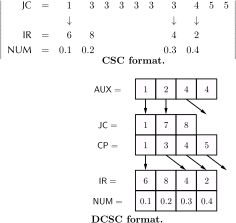
\includegraphics{DCSCvsCSC.svg.png} \label{fig:DCSCvsCSC}
\end{figure}

\subsection{Moltiplicazione tra matrici ipersparse rappresentate con DCSC}
\label{ssec:hypersparseGEMM}
Segue la descrizione di un algoritmo risolutivo per la moltiplicazione tra matrici
ipersparse \parencite{2dNewIdeas}, basato su una formulazione outer-product ed
utilizzato in alcuni algoritmi SpGEMM.\\
lo pseudo-codice dell'algoritmo è riportato in \ref{figCode:hypersparseGEMM} 


{\bf fase di preprocessamento} \\
viene effettuata una trasposizione di B, così da avere un indicizzamento rapido delle righe di B
in formato DCSC, necessario per la
formulazione outer-product.\\ %costo di trasposizione varia tra $O(n + nnz(B) \to nnz(B) lg nnz(b)) in base all implementazione
Viene effettuata l'intersezione tra gli indici delle colonne non zero di A e
delle righe non zero di B, identificando così il set $Isect = A.JC \cap B^T.JC$ degli
indici che partecipano all'outer-product.\\
\\
Successivamente vengono effettuati $|Isect|$ prodotti cartesiani \ref{fig:hypersparseGEMMGraphical} 
generanti matrici $a_{*i} \cdot b_{i*}$, i cui elementi è possibile mettere in biiezione 
con la lista di indici $(r_{id},c_{id})$ derivante dal prodotto cartesiano tra gli indici
di riga non zero della colonna i-esima di $B^T$ e gli indici di riga non zero 
della colonna i-esima di $A$.\\
La matrice risultante C può essere ottenuta mediante l'unione di queste liste,
sommando i contributi degl'elementi aventi gli stessi indici in liste
diverse.\\
Per implementare la costruzione di C dagli outer-products
è utilizzata una coda con priorità contenete elementi relativi ai
prodotti cartesiani per le colonne di $A$ e le colonne di $B^T ~\in~ Isect$, 
aventi per chiave $(r_{id},c_{id})$ e per valore il prodotto relativo e l'indice
della colonna di $A$ o $B^T$ relativa.\\
Verrà ripetutamente estratto il minimo dalla coda e reinserito
l'elemento successivo dalla lista di indici di relativa, sommando i
contributi di elementi con la stessa chiave.
I risultati verranno accumulati in uno stack mediante una rappresentazione
matriciale a coordinate degli elementi % TODO CHECK COO LIKE STACK ACCUMULATE
per poi essere convertiti nella matrice finale C in formato DCSC.\\

La complessità computazionale dell'algoritmo è $O(nzc(A) + nzr(B) +flops \cdot lg( ni))$
dove $ni$ è la dimensione della coda con priorità e $flops$ è il numero di
operazioni aritmetiche necessarie per il prodotto di A e B.\\

\begin{figure}[h]
  \centering \includegraphics{hypersparseGEMM.svg.png}
  \caption[Algoritmo sequenziale per SpGEMM tra matrici ipersparse] \decoRule \label{figCode:hypersparseGEMM}
\end{figure}

\begin{figure}[h]
  \centering 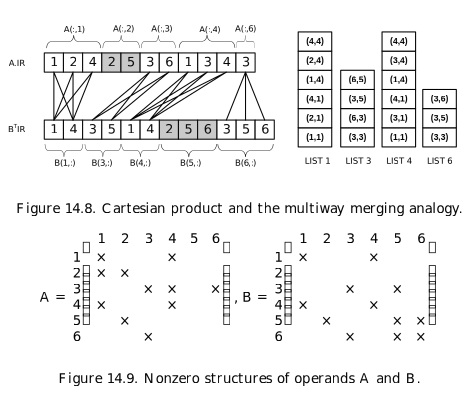
\includegraphics{hypersparseGEMMGraphical.svg.png}
  \caption[Rappresentazione grafica del prodotto cartesiano 
   a supporto di hypersparseGEMM ] \decoRule \label{fig:hypersparseGEMMGraphical}
\end{figure}


\subsection{2D}

\subsubsection{Derivati di Gustavson} \label{ssec:gustavsonDerivate}
Una parallelizzazione della formulazione per righe dell'algoritmo di Gustavson è
descritta in \parencite{intelSpGEMMDenseAccumulator}, sfruttando la
rappresentazione di matrici sparse in formato CSR. 
Lo pseudocodice dell'algoritmo è riportato in \ref{figCode:gustavsonRigheBlocksIntel}
e una sua rappresentazione grafica è raffigurata in
\ref{fig:gustavsonRigheBlocksGraphicalIntel}\\
%Partizionamento = Gustvason a blocchi
Viene effettuato un partizionamento delle righe di A e delle colonne di B e 
coppie di partizioni corrispondenti vengono utilizzate per calcolare un
blocco bidimensionale della matrice risultante C.\\
%accumulatore denso X
In accordo con la formulazione per righe dell'algoritmo di Gustavson, vengono
accumulati i contributi degli elementi \nnz delle righe di A e corrispettive porzioni
delle righe di B relative al calcolo di un blocco di C. 
Per effettuare efficientemente questa operazione, i vettori sparsi risultanti
dalle iterazioni dell'algoritmo, vengono accumulati in vettore denso X, 
semplicemente sommandone le componenti \nnz nelle relative locazioni di X.\\
%alternative memory efficient con overhead
In questa formulazione del problema, una soluzione di accumulazione 
alternativa potrebbe essere quella di accumulare i contributi per una riga di C 
utilizzando una hash-table di elementi aventi per chiave l'indice di colonna. 
Tuttavia, quest'approccio ha lo svantaggio di avere l'overhead relativo alla 
computazione delle funzioni hash e gestione di eventuali liste di collisione.\\
%implementazione conversione
Al termine del calcolo di una riga di un blocco di C, l'accumulare X viene
convertito in una riga CSR con l'ausilio di un ulteriore vettore di indici di
elementi \nnz sommati in X.\\
%Nota su partizionamento -> MENO cache miss su X
Utilizzando un partizionamento delle colonne di B è possibile partizionare anche
l'accumulatore X relativo ad una riga risultante di C. In questa maniera si
riduce il numero di cache line toccate dagl'aggiornamenti di X, riducendo il
numero di cache miss relativi al ciclo interno dell'algoritmo.\\
Gli autori dell'algoritmo hanno verificato la riduzione di cache miss
utilizzando degli hardware counter per verificare il numero di cache miss L2
(tipicamente catturati dalla cache LLC) al variare del partizionamento di B % TODO QUANTIFICAZIONE?
%%Valutazione sul partizionamento di B -> X
%svantaggi
Tuttavia il partizionamento di B in rappresentazioni CSR separate, 
oltre che comportare un overhead computazionale, può comportare svantaggi in
termini di banda di memoria durante la lettura dei blocchi di B, che possono
essere notevolmente più sparsi della matrice originaria. %TODO link a ipersparse
%quantificazione euristica beneficio
Un beneficio dal partizionamento di B e di X, contro gli overhead citati, è
presente quando si ha certezza che per una significativa porzione delle righe
risultanti di C, l'occupazione dei \nnz, corrispondenti agli aggiornamenti
dell'accumulatore X, è maggiore della dimensione della cache L2.\\
Per quantificare il numero di \nnz nelle righe risultanti di C viene utilizzata
una metrica basata sulla stima di \nnz in $c_{i*}=e\_nnz(i)$ di
\parencite{intelSpGEMMDenseAccumulator} %TODO SOURCE ARTICLE OF ESTIMATE
dove si partiziona B se
$e\_nnz = \frac{\sum\limits_{i:e\_nnz(i) > L2\_FP\_WORDS} e\_nnz(i)}
{\sum\limits_{i=1}^m e\_nnz(i)} ~>~0.3$\\
%TODO scheduling dinamico -> load balancing con perizioni piccole t.c. #partizioni = 6-10 X #threads
\begin{figure}[h]
  \centering 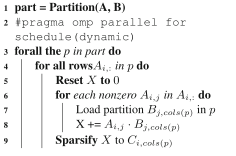
\includegraphics{gustavsonRigheBlocksIntel.svg.png}
  \caption[adattamento parallelo dell'algoritmo di Gustavson] \decoRule \label{figCode:gustavsonRigheBlocksIntel}
\end{figure}
\begin{figure}[h]
  \caption[rappresentazione grafica dell'adattamento parallelo dell'algoritmo di Gustavson] 
  \centering \includegraphics{gustavsonRigheBlocksGraphicalIntel.svg.png} \label{fig:gustavsonRigheBlocksGraphicalIntel}
\end{figure}

\subsubsection{Dense SUMMA} %versione base C=AB
Un partizionamento bidimensionale della risoluzione del prodotto tra matrici
dense è realizzato dell'algoritmo parallelo SUMMA \parencite{denseSumma} che è alla
base di una sua controparte per matrici sparse \parencite{sparseSUMMA}.\\
Il calcolo di $C=AB$ è sudiviso in sottomatrici assegnate a processi organizzati 
in una griglia bidimensionale di dimensione  $p_r x p_c$.\\
È possibile calcolare un blocco della matrice C come:
$C_{ij} =  \overbrace{\left(  A_{i1} | \dots |  A_{ip_c} \right)}^{\tilde{A^{i*}} }
~\cdot~ \overbrace{\left( 
        \begin{array}{c} B_{1j} \\ \vdots \\  B_{p_r j}
        \end{array} \right)} ^{\tilde{B^{*j}}} $\\
dove si usa la notazione:
\begin{itemize}
  \item $\tilde{a_{*l}}^{i*} \in \tilde{ A^{i*}}$ rappresenta 
    la colonna l-esima nella riga i-esima nella decomposizione a blocchi di A
  \item $\tilde{b_{l*}}^{*j} \in  \tilde{B^{*j}}$ rappresenta 
    la riga l-esima nella colonna j-esima nella decomposizione a blocchi di B.
\end{itemize}  
Applicando la formulazione outer-product su $\tilde{ A^{i*}}$ e $\tilde{B^{*j}}$
si ha che $C_{ij}=\sum\limits_{l=1}^{k}\tilde{a_{*l}}^{i*} \cdot \tilde{b_{l*}}^{*j}$\\
Considerando un partizionamento delle matrici in sottomatrici all'interno della
griglia di processi %assegnate in maniera tale che  ... 
si può eseguire l'operazione GEMM in parallelo come riportato dallo pseudocodice
in \ref{figCode:denseSUMMA}\\
\begin{figure}[h]
  \centering 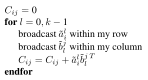
\includegraphics{denseSUMMA.svg.png}
  \caption[esecuzione dense SUMMA sul processo $P_{ij}$] \decoRule \label{figCode:denseSUMMA}
\end{figure}
Nell'articolo originale vengono discussi miglioramenti a questa formulazione
basati su uno scambio di dati tra i processi in un sistema a memoria distribuita
mediante una comunicazione ad anello 
riformulazione del calcolo di $C_{ij}$ utilizzando blocchi di
colonne di $\tilde{ A^{i*}}$ e righe di $\tilde{B^{*j}}$.\\

\subsubsection{Sparse SUMMA}
Un partizionamento bidimensionale del problema SpGEMM è realizzato
dall'algoritmo Sparse SUMMA \parencite{sparseSUMMA}, derivato dalla sua
controparte per matrici dense.\\
%SPARSE SUMMA
È riportato lo pseudo-codice dell algoritmo sparseSUMMA 
in \ref{figCode:sparseSUMMA} e una sua iterazione graficamente in
\ref{fig:sparseSUMMAIteration}.\\
Le matrici sono divise in blocchi e rappresentante in formato DCSC,
trasponendo la matrice B per avere un indicizzamento rapido delle sue righe.\\
Procedendo in blocchi di colonne di una sottomatrice di A e della corrispettiva
sottomatrice di $B^T$, lungo la dimensione comune di A e B,
vengono calcolati in parallelo le sottomatrici $C_{ij}$, 
utilizzando l'algoritmo hypersparseGEMM \ref{ssec:hypersparseGEMM}.\\
Il costo computazionale dell'algoritmo è 
$O(\frac{dn}{\sqrt{p}}+\frac{d^2n}{p}lg(\frac{d^2n}{p}))$
%TODO CONSIDERAZIONE SU EFFICIENZA ALLO SCALARE DI p ... cmq no speedup bounds!
\begin{figure}[h]
  \caption[SparseSUMMA, per una risoluzione parallela di SpGEMM con un partizionamento 2D]
  \centering \includegraphics{sparseSUMMA.svg.png} \decoRule \label{figCode:sparseSUMMA}
\end{figure}
\begin{figure}[h]
  \caption[esecuzione di un iterazione dell'algoritmo sparseSUMMA]
  \centering \includegraphics{sparseSUMMAIteration.svg.png} \decoRule \label{fig:sparseSUMMAIteration}
\end{figure}

\subsection{3D}
Un partizionamento tridimensionale del problema SpGEMM è realizzato dall'
algoritmo Split-3D-SpGEMM \parencite{Split3DSpGEMM}, dove al partizionamento
bidimensionale descritto precedentemente, viene aggiunto una ulteriore
suddivisione delle sottomatrici in blocchi nella terza dimensione della griglia di processi.
%TODO CONSIDERAZIONI su overhead mem per C -> sparsity-structure dependent ->
%sfruttabile bene la sparsità del risultato in meno occupazione di memoria
Il partizionamento delle matrici è rappresentabile sul cubo di lavoro W come
riportato in figura \ref{fig:workCube3D}, dove il processo P(i,j,k) possiede la
porzione della matrice di A: 
$A(im/p_r:(i+1)m/p_r - 1, jn/p_c + kn/(p_c p_l ) : jn/p_c + (k + 1)n/(p_c p_l) - 1)$  \\
\begin{figure}[h]
  \caption[rappresentazione 3D della suddivisione della computazione SpGEMM]
  \centering \includegraphics{workCube3D.svg.png} \decoRule \label{fig:workCube3D}
\end{figure}
L'algoritmo è riportato nello pseudo-codice \ref{figCode:Split3DSpGEMM} e una
sua iterazione è raffigurata graficamente in \ref{fig:Split3DSpGEMMIteration}.\\

In maniera simile al caso di sparseSUMMA %TODO \ref{sparseSummaDescriptionStart}
si procede in parallelo calcolando il prodotto di sottoblocchi corrispondenti
alle sottomatrici di A e B, accumulando risultati intermedi la cui collocazione
è relativa all'intera fiber W(i,j,:).
Infine i risultati intermedi dei processi P(i,j,:), vengono distribuiti lungo la fiber
W(i,j,:), sommando i contributi relativi agli stessi indici.
\begin{figure}[h] 
  \caption[Split3DSpGEMM, per una risoluzione parallela di SpGEMM con un partizionamento 3D
     nel caso semplificato di una griglia di processi $\sqrt{p/c}~x~\sqrt{p/c}~x~c$]
  \centering \includegraphics[width=1.0\textwidth]{Split3DSpGEMM.svg.png} \decoRule \label{figCode:Split3DSpGEMM}
\end{figure}
\begin{figure}[h]
  \caption[esecuzione di un iterazione dell'algoritmo Split3DSpGEMM]
  \centering \includegraphics[width=1.0\textwidth]{Split3DSpGEMMIteration.svg.png} 
  \decoRule \label{fig:Split3DSpGEMMIteration}
\end{figure}














%%Figure options
%%h 	Place the float here, i.e., approximately at the same point it occurs in the source text (however, not exactly at the spot)
%%t 	Position at the top of the page.
%%b 	Position at the bottom of the page.
%%p 	Put on a special page for floats only.
%%! 	Override internal parameters LaTeX uses for determining "good" float positions.
%%H 	Places the float at precisely the location in the LaTeX code. Requires the float package, though may cause problems occasionally. This is somewhat equivalent to h!.
